\subsection{Similie}\label{sec:similie}
\par
Simile is a visual modelling environment, developed originally for the dynamic modelling of ecological and environmental systems, which supports a wide range of ways of representing space, it combines a System Dynamics and an object-based approach. System Dynamics is based on a conceptualisation of dynamic systems in terms of stocks and flows, variables and influences. \autocite{dsl:simile-simulistics}
\par
Like many other modelling frameworks or software tools, simile supports component-based modelling, which helps to divide a complex system to small modulars, as well as System Dynamics modelling, which is a methodology, mainly used to analyze complex mathematical models and problems. Simile is already a successful modelling software, and it has already been adopted in various scientific researches of agricultural or geographical fields in many different countries. With Simile, model developers are also able to integrate knowledges from various studies, guide the research processes and make prediction. Besides that, they can also share the models they have created over the internet, since the models are save as a text file with a structured format. \autocite{dsl:simile-muetzelfeldt} It means that the models created by Simile may be reusable by other modelling framework for further development.
\subsubsection{Technical implementation}
\par
Simile is capable of handling different modelling types, which are most commonly used by model developers, such as system dynamics, object oriented models, modular models, population dynamics models, etc. \autocite{dsl:simile-simulistics} It comes up with a set of low-level primitive modelling elements that enable various types of models to be constructed, without using the terms and concepts individually associated with each model type. \autocite{dsl:simile-muetzelfeldt} The simile modelling language consists of 12 basic modelling elements. In this chapter, we will focus on how these elements can be applied to system dynamics and modular modelling.
\par
As we have mentioned above, system dynamic methodology is used to simulate and analyze the behaviors of a complex system. To demonstrate a system dynamic scenario, we often use a stock and flow diagram, which presents the relationship between the volume of a stock and the flows coming into or out of the stock. The volume of the stock accumulates or depletes over time, because of the incoming and outgoing flows. The basic modelling elements from Simile can handle this kind of modelling and provide a visualization tool for users to analyze the changes of the stock in a quantitative way. Simile provide four modelling elements for system dynamics: compartment, flow arrow, variable and influence arrow. The compartment element is used to describe a stock and its status, such as the credit of a bank account, the amount of water volume, etc. Each compartment element of simile should be initialize with a numeric value, which could be calculated with other variables or constants. The flow arrow is visually represented by an incoming or outgoing arrow of a compartment. They cause the increment and decrement of the amount of substances in the compartment. The flow arrow may also connect two different compartment, which means that the substances of one compartment will flow into another compartment. The value of the flow arrow can be a constant or a mathematical expression. The variable element of simile contains a value of a constant or a function. In Simile modeling environment, it serves as a parameter, an intermediate variable, an output variable, etc, for example, it can be the input or output parameter of a component. The influence flow connects two different modeling elements. It represents that the value of one element will be used to calculate the other.
\par
The following figure shows how a simple system dynamic model in Simile looks like.
\begin{figure}[h]
	\centering
	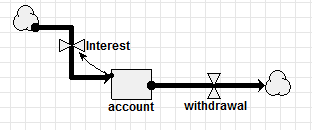
\includegraphics[width=0.7\textwidth]{pics/simile/simile_example_bank_account.png}
	\caption{System Dynamics Model Bank Account in Simile \label{fig:simile_example_bank}}	
\end{figure}
\par
Figure \ref{fig:simile_example_bank} represents a simple bank account modeled by compartment, flow arrow and influence arrow. The rectangle in the middle of the model is a compartment, which represents a bank account. The incoming flow arrow represents the interests of the bank account, which will increase the credit of the account. , In the opposite, the outgoing flow arrow describes the withdrawal of the bank account, which will decrease its credit. The influence flow starting from account to Interest indicates that the value of the interest depends on the total credit of the account.
\par
Furthermore, Simile provides a tool for us to simulate and visualize our model. In this tool, there are some settings, which help us to control the result and the visualization (see the left panel of figure \ref{fig:simile_example_evaluatin}). The “Execute for:” setting defines how often do we want to execute the model. The “current time:” setting defines the current calculation point. The “plus” button in the right panel defines the parameter that we need to analyze in the vertical axis of the visualization diagram. The curve in the diagram of the right panel shows us how the value of bank account changes over time. With this diagram, we are able to predict the trend of the credit changes of the bank account.
\begin{figure}[h]
	\centering
	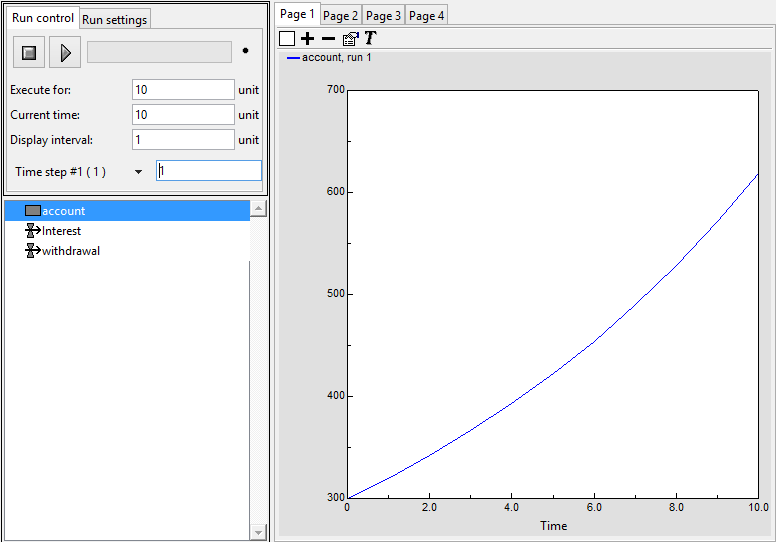
\includegraphics[width=0.8\textwidth]{pics/simile/simile_example_evaluating_model.png}
	\caption{Running and evaluating the model \label{fig:simile_example_evaluating}}	
\end{figure}
\par
An existing Simile model can be used as a submodel by other models. Simile software also provides a modelling element to represent a submodel.  A number of modelling elements can be grouped together to form a submodel. We can either create a blank submodel and add other modelling elements into the submodel, or we can draw the submodel to surround an existing model. Model developers can make links between two sub-components with variable elements. The variable elements are the outputs of one sub-component and they are input parameters for the other sub-component. The output of one component is required by the other. Through combining small sub-components together, modellers can build up a large complex system.
\par
Figure \ref{fig:simile_example_submodel} shows an example of creating a submodel using Simile. This example extends the system dynamic model of a bank account by surrounding the existing system dynamic model with a rectangular and adding input and output variables to the submodel. The component bank account should now make use of an external input of interest rate to calculate the current interest. The value of ``interest\_rate'' variable should be provided by other components. The bank account also provides an output variable ``status'', which represents the current credit of the account. This output variable can be used by other components. Through the input and output variables, the bank account component can be connected with other components to make up a larger submodel.
\begin{figure}[h]
	\centering
	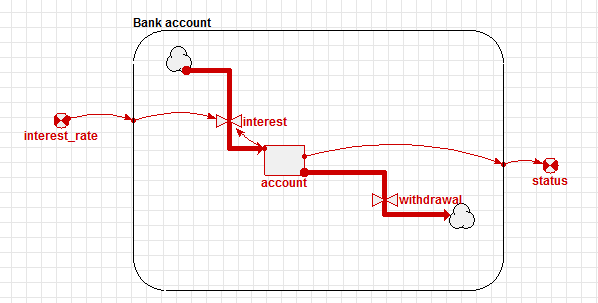
\includegraphics[width=0.8\textwidth]{pics/simile/simile_example_submodel.png}
	\caption{Submodel example bank account modular \label{fig:simile_example_submodel}}	
\end{figure}
\par
The Simile modelling tool supports much more modelling types, other than system dynamics and modular modelling, such as disaggregation, spatial modelling, population modelling, object based modelling, etc. For further information about these modelling types, please refer to the homepage of the Simile software, or the paper \autocite{dsl:simile-know}.
\subsubsection{Advantages of Simile}
\par
The Simile modelling software offers the following benefits to the model developers:

\begin{itemize}
\item 
The user-friendly graphic interface gives the model developers an effective and intuitive way to create models. It helps to save time and improves the quality and reliability of the created models.
\item
It simplifies documentation of models. The Simile models are largely self-documented by simply attaching comments to model elements. \autocite{dsl:simile-muetzelfeldt} This feature avoids the inconsistency between documents and models. 
\item
Simile allows models to be saved to files and loaded from files. This feature improves the reusability of submodels and makes testing of submodel easier, since a submodel can be separated from the whole model and saved to a new file. In this way, the separated submodel will be regarded as a stand-alone model and possible existing problems are easier to identify.
\item
Compared to other System Dynamics modelling environments, Simile is able to specify multiple instances of an entity. \autocite{dsl:simile-muetzelfeldt} Unlike the conventional way to create an array that holds some instances of a submodel, Simile simply groups existing modelling elements together for a submodel and then specify the instances of these submodels.
\item 
Simile has the ability to link elements declared in the model with entities declared in distributed ontologies, thus reducing the risk of ambiguities and misuse of data, which are quite frequent in this modelling framework.
\end{itemize}

\subsubsection{Disadvantages of Simile}
\par
Despite of the advanced features of Simile, it also comes with some disadvantages:
\begin{itemize}
\item 
The Simile models need to adhere to a standard and common declarative modelling language, which currently exists only in some domains.
\item
Although Simile provides several primitive modelling elements for generic modelling, it is still desirable, that more experienced model developers could work at a lower level to allow different domain-specific language to be combined in one model. The conceptual gap between modellers and the modelling language should be narrowed. \autocite{dsl:simile-muetzelfeldt}
\item
Simile does not reflect all the properties of object oriented component based modelling.  In Simile, all attributes and variables of a subcomponent are visible to users. This violates terms of object oriented modelling, since some attributes should be hidden to the external world, or the access should be restricted. Furthermore, Simile models does not have concepts of inheritance and specialization. \autocite{dsl:simile-muetzelfeldt}
\item
The Simile models are currently not able to be seamlessly integrated with a geographic information system.  Compatible problems have to be solved.
\item 
It lacks of plenty of models over the internet for users to download. It is difficult for model developers to search for suitable models in the internet for study and further development.
\end{itemize}





















